\documentclass{article}

\usepackage[utf8]{inputenc}
\usepackage[T1]{fontenc}
\usepackage{geometry}
\usepackage{graphicx}   %ALLOWS INSERTING IMAGES (AND MAYBE SOME MORE STUFF) %
\usepackage{subcaption} %ALLOWS CAPTIONS FOR SUBFIGURES%
\usepackage{verbatim} % ALLOWS MULTILINE COMMENTS WITH \begin{comment} AND \end{comment} %
\usepackage{amsmath,amssymb} % PERMETTE L'USO DI SIMBOLI MATEMATICI "AVANZATI" COME 'MINORE O UGUALE' E ALTRI %
\usepackage{amstext}
\usepackage{enumitem} %PERMETTE L'USO DI ELENCHI NUMERATI

\geometry{a4paper}
                        %Una riga vuota tra due scritte spazia di una riga anche sul pdf. Andare a capo una volta non provoca nulla nel pdf%
\usepackage[italian]{babel}
%\usepackage[french, italian]{babel} non funzione per motivi a me ignoti
\frenchspacing 

%%%  INTESTAZIONE  %%%

\title{Relazione dell'esperimento di misura della velocità della luce}
\author{Lorenzo Ramella, Alessandro Matteo Rossi, Marco Tambini}
\date{\today}


%%%  INIZIO DOCUMENTO  %%%

\begin{document}
\maketitle

%%%  ABSTRACT  %%%

\begin{abstract}
L’esperimento si propone di misurare la velocità delle luce usando il metodo di Focault. %%da modificare
\end{abstract}

%%%  INDICE  %%%%

\tableofcontents
\newpage

%%%  INTRODUZIONE TEORICA  %%%

\section{Introduzione teorica}
Il metodo di Focault per la misura della velocità della luce consiste nell'uso di uno specchio rotante, che riflette la luce emessa da una sorgente su di uno specchio 
concavo. 

Una sorgente luminosa $S$ emette una luce che, opportunamente diaframmata da una lente $L_1$, attraversa una lastra semitrasparente angolata di 45° rispetto alla 
direzione del fascio. Una lente $L_2$ focalizza il fascio nel punto $S'$ sullo specchio concavo, dopo essere stata deflessa dallo specchio rotante. La luce riflessa 
dallo specchio concavo viene deflessa nuovamente dallo specchio rotante, che nel frattempo ha ruotato di un angolo 

\begin{equation}
\alpha = \omega \frac{2D}{c}
\end{equation}

dove $\omega$ è la velocità angolare dello specchio e $D$ è la distanza tra lo specchio rotante e lo specchio concavo.

Il fascio luminoso di ritorno sulla lente $L_2$ viene focalizzato come se provenisse da una sorgente $S''$ spostata da $S'$ di una quantità 

\begin{equation}
\Delta = 2 \alpha D
\label{DELTA}
\end{equation}

Tenendo presente che il fattore di amplificazione $G$ della lente $L_2$ è esprimibile mediante la seguente relazione:

\begin{equation}
G=\frac{b}{D+a}
\label{G}
\end{equation}

dove $b$ è la distanza tra $L_2$ e la sorgente luminosa e $a$  la distanza tra $L_2$ e lo specchio rotante. Lo spostamento laterale $\delta$ dell'immagine si ottiene quindi
combinando le equazioni (\ref{DELTA}) e (\ref{G})
\begin{equation}
\delta = G\Delta =\frac{2\alpha b D}{D + a}=\frac{4 D^2 b \omega}{c(D+a)}
\label{delta}
\end{equation}

È possibile ricavare $b$ dalla legge dei punti coniugati. Sapendo che:

\begin{equation}
\frac{1}{b}+\frac{1}{D+a}=\frac{1}{f_2}
\label{punticoniug}
\end{equation}

Si deduce che:

\begin{equation}
b=\frac{f_2(D+a)}{D+a-f_2}
\end{equation}

E quindi, conoscendo l'espressione di $\delta$ dalla equazione (\ref{delta}), in cui compare $c$, e avendo ricavato l'unica variabile incognita $b$ dall'equazione
(\ref{punticoniug}), si ottiene:

\begin{equation}
c = \frac{4f_2D^2(\omega-\omega_0)}{[(D+a+f_2)\Delta\delta]}
\end{equation}

dove $\omega_0$ è la velocità angolare iniziale e $\Delta\delta = \omega - \omega_0$ è lo spostamento dell'immagine della sorgente luminosa.

\begin{figure}[h]
    \centering
        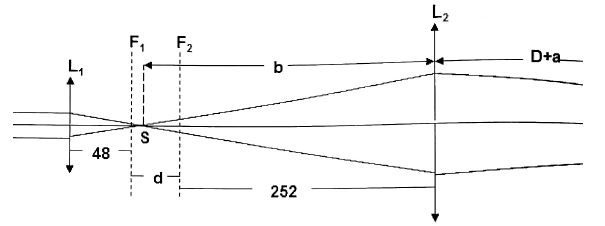
\includegraphics[width=0.6\linewidth]{IntroTeorica1.JPG}
    \caption{Schema apparato - intorno del beam-splitter}
\end{figure}

%%%  PROGETTAZIONE DELL'ESPERIMENTO  %%%

\newpage

\section{Progettazione dell'esperimento}

\begin{figure}[h] %here, top, bottom, ! = forza posizionamento dove latex riesce, H mettilo dove cazzo dico io%
    \centering
    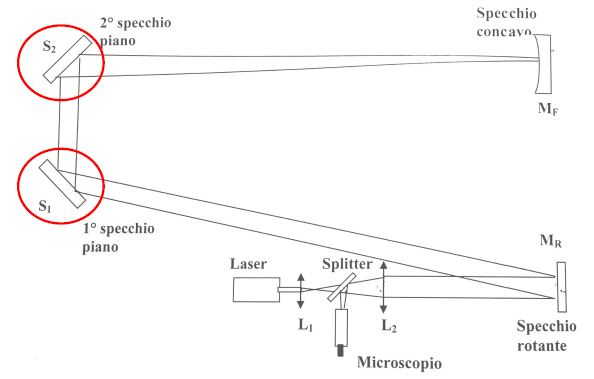
\includegraphics[width=0.6\linewidth]{Progettazione1.JPG}
    \caption{Schema dell'apparato di laboratorio}
    \label{schema_apparato}
\end{figure}

Il banco ottico di laboratorio era composto da una sorgente luminosa e un sistema di lenti e specchi, il tutto ancorato saldamente alle varie parti del banco mediante 
morse.

Prima di cominciare le misure di $c$ è necessario assicurarsi che gli elementi del banco ottico siano correttamente posizionati.

\vspace{3mm}

Per fare ciò principio abbiamo misurato la lunghezza del cammino ottico $D$ del raggio luminoso dallo specchio rotante allo specchio concavo. Per fare ciò abbiamo raccolto 
4 misure per le distanze tra specchio rotante e specchio 1 $d_{rot,1}$, tra specchio 1 e specchio 2 $d_{1,2}$ e tra specchio 2 e specchio concavo $d_{2,conc}$, per poi 
ottenere tramite una somma delle loro medie aritmetiche (con incertezza $\sigma d = \sigma D = 0,01 m$) il valore di $D$. Gli strumenti utilizzati in questa fase sono
stati due rotelle metriche di portata $15m$ e $3m$.

Come mostrato in Figura \ref{schema_apparato}, la sorgente luminosa coerente è un laser A CHE COSA?? fissato magneticamente a un binario graduato. Per evitare danni agli
occhi abbiamo adoperato una coppia di lamine polaroid, con base magnetica, poste sul binario subito dopo il laser.
è necessario porre una prima lente $L_1$ $70 mm$, seguendo la scala graduata con la sensibilità del millimetro, per poter fare convergere la luce proveniente "dall'infinito"
\begin{comment}(le dimensioni lineari della lente sono molto ridotte rispetto alla distanza tra laser e $L_2$)\end{comment} alla sua distanza focale, che il produttore 
della lente dichiara essere a una distanza $f_1 = 0,048 m$. A una distanza di $180mm$ dall'inizio della scala graduata è posto il beam-splitter, un elemento dotato di uno
specchio semiriflettente orientato a 45° rispetto alla luce incidente, che permette di trasmettere la luce in arrivo alla lente $L_2$. La lente $L_2$, con 
focale dichiarata dal produttore di $f_2=0,252m$, è posta a distanza $b = ???$ dal beam-splitter e trasmette a sua volta la luce allo specchio rotante. 
Questo sistema di lenti serve per ottenere un'onda piana, e questo è possibile poichè la somma delle focali di $L_1$ ed $L_2$ è maggiore della loro distanza. 


Per permette alla luce di percorrere il sistema di specchi che va dallo specchio rotante, allo specchio $S'$, quindi allo specchio $S''$ e infine allo specchio concavo 
bisogna inizialmente accertarsi, posizionando una squadretta forata con base magnetica sul binario, che la luce incida sul centro dello specchio rotante.
Contemporaneamente bisogna agire sulla cinghia dello specchio rotante per permettere al raggio incidente di raggiungere la parte riflettente dello specchio e quindi 
subire una riflessione verso il centro (approssimativamente) di $S'$.
Fatto questo si regola l'inclinazione di $S'$ per riflettere il raggio proveniente dallo specchio rotante approssimativamente nel centro di $S''$, attraverso due
viti micrometriche poste dietro lo specchio. Si ripete quest'ultimo procedimento per portare il raggio dal centro di $S''$ al centro dello specchio concavo.

Specifichiamo che a causa della complessità della misura della focale di una lente le focali e le posizioni corrette per lenti e beam-splitter vengono fornite dai 
docenti, e le consideriamo affette da un'incertezza sistematica trascurabile.

\vspace{3mm}

Raggiunta la condizione di raggio che percorre tutta la lunghezza $D$, è necessario agire nuovamente sulle viti micrometriche degli specchi per fare tornare il raggio
luminoso indietro fino al beam-splitter ripercorrendo il suo cammino di andata. Può essere in questa fase utile utilizzare un foglio di carta millimetrata da posizionare
a mezz'aria dove si pensa che i raggi passino, per verificare spostandolo sempre più verso lo "specchio di destinazione" che i raggi coincidano e che il puntino luminoso
del raggio di andata non si discosti da quello del raggio di ritorno.

\vspace{3mm}

\underline{Problemi tecnici riscontrati:} 

Sebbene sia abbastanza agevole misurare le distanze tra specchi, posizionare le lenti e il beam-splitter e fondamentale già da questa prima fase prestare la 
/underline{massima attenzione} a non toccare il banco di lavoro (singolare, sebbene $S'$ e $S''$ fossero posti su un secondo tavolo, il che rendeva utile misurare alcune
distanze con la rotella di portata $15m$). 
Questo potrebbe compromettere gravemente la taratura del banco.

È invece complicato e dispendioso a livello di tempo correggere la posizione degli specchi. Infatti mentre uno dei due sperimentatori lavorava sulle viti micrometriche,
l'altro aveva il compito di tracciare il percorso del raggio o osservandone la posizione sulle pareti (se e quando possibile) o aiutandosi con la carta millimetrata 
quando esso era prossimo a raggiungere il centro dello specchio.

Il compito certamente più arduo è fare ritornare il raggio di ritorno su quello di andata, poichè la carta millimetrata è l'unico strumento valido. Durante il suo utilizzo
il rischio di coprire il raggio di andata (facendo scomparire quello di ritorno) nel tentativo di vederli entrambi sul bordo del foglio è alto.

%%%  MISURE  %%%

\section{Misure}

\subsection{Raccolta dati}
L'esperienza è stata svolta da Rossi in collaborazione con Tambini e Ramella in collaborazione con ?????. Si è deciso di analizzare i due set di misure, fino al calcolo 
della miglior stima della velocità della luce $c_{best}$, separatamente. Questo a causa di differenze:

\begin{enumerate}
    \item Sulla misura di $D$ poichè sono stati usati due apparati dello stesso modello ma fisicamente differenti, e quindi si sono presentate differenze.
    \item Sul motore dello specchio rotante utilizzato. Il gruppo Rossi-Tambini ha utilizzato un motore per lo specchio rotante che permetteva solo la regolazione in 
            senso orario e antiorario con una frequenza di rotazione di $\nu = 1500 Hz$ e $\nu = 750 Hz$. Mentre il motore del gruppo Ramella-??? permetteva una rotazione
            oraria e antioraria con frequenza variabile fino a circa i $1500 Hz$.
\end{enumerate}

\subsection{Analisi dati - Misure Rossi-Tambini}

\subsection{Analisi dati - Misure Ramella-???}

\section{Calcolo c\begin{footnotesize}\textsubscript{BEST}\end{footnotesize}} %SIMPY

\section{Conclusioni}

\section{Appendice}



\end{document}


% Å ^{\circ} \vspace{1mm} per spaziare verticalmente \begin{equation} e \end{equation} con dentro un \label e fuori un \ref per numerare e avere il riferimento alle
% equazioni È


